\chapter{认识 PIE-Block}
\label{ch:concise-intro}

\begin{introduction}
  \item 了解 PIE-Block 的定位与四种项目类型；
  \item 会新建、打开与保存项目；
  \item 记住从配置到烧录的通用流程与安全前提。
\end{introduction}

\section{软件定位}

PIE-Block 是面向首都师范大学 RoboMaster 校内赛的机器人图形化配置集成开发环境，运行于
Windows 与 Linux 桌面端。软件把“让机器人按预期动作”拆成一组可以照做的步骤：在向导中
选择项目类型，按硬件方案填写参数，软件检查配置、生成主控程序、完成编译，最后通过 USB
把固件写入主控板。整个过程不需要编写程序，也不需要自行搭建编译环境。

所有工作围绕 \texttt{.pieproj} 项目文件展开。配置每变化一次，软件自动保存，界面右上角
显示“已保存”；关闭软件后重新打开项目，会回到上次离开的步骤。

\section{四种项目类型}

从首页“新建项目”选择四种类型之一，如表~\ref{tab:concise-kinds} 所示。

\begin{table}[htbp]
  \centering
  \small
  \begin{tabularx}{\linewidth}{@{}>{\raggedright\arraybackslash}p{0.16\linewidth}
      >{\raggedright\arraybackslash}p{0.34\linewidth}
      >{\raggedright\arraybackslash}X@{}}
    \toprule
    项目类型 & 用途 & 向导页面 \\
    \midrule
    步兵 & 底盘、云台、拨弹与摩擦轮的标准战斗构型 & 遥控器与底盘、云台与拨弹、控制与摩擦轮 \\
    工程 & 自定义底盘、机械臂、多套控制模式 & 遥控器与底盘、PWM 与引脚、模式切换、动作映射 \\
    调试 & 装车前逐路检查输出 & 测试序列 \\
    音乐 & 用蜂鸣器演奏乐曲 & 钢琴卷帘 \\
    \bottomrule
  \end{tabularx}
  \caption{四种项目类型}
  \label{tab:concise-kinds}
\end{table}

\begin{figure}[htbp]
  \centering
  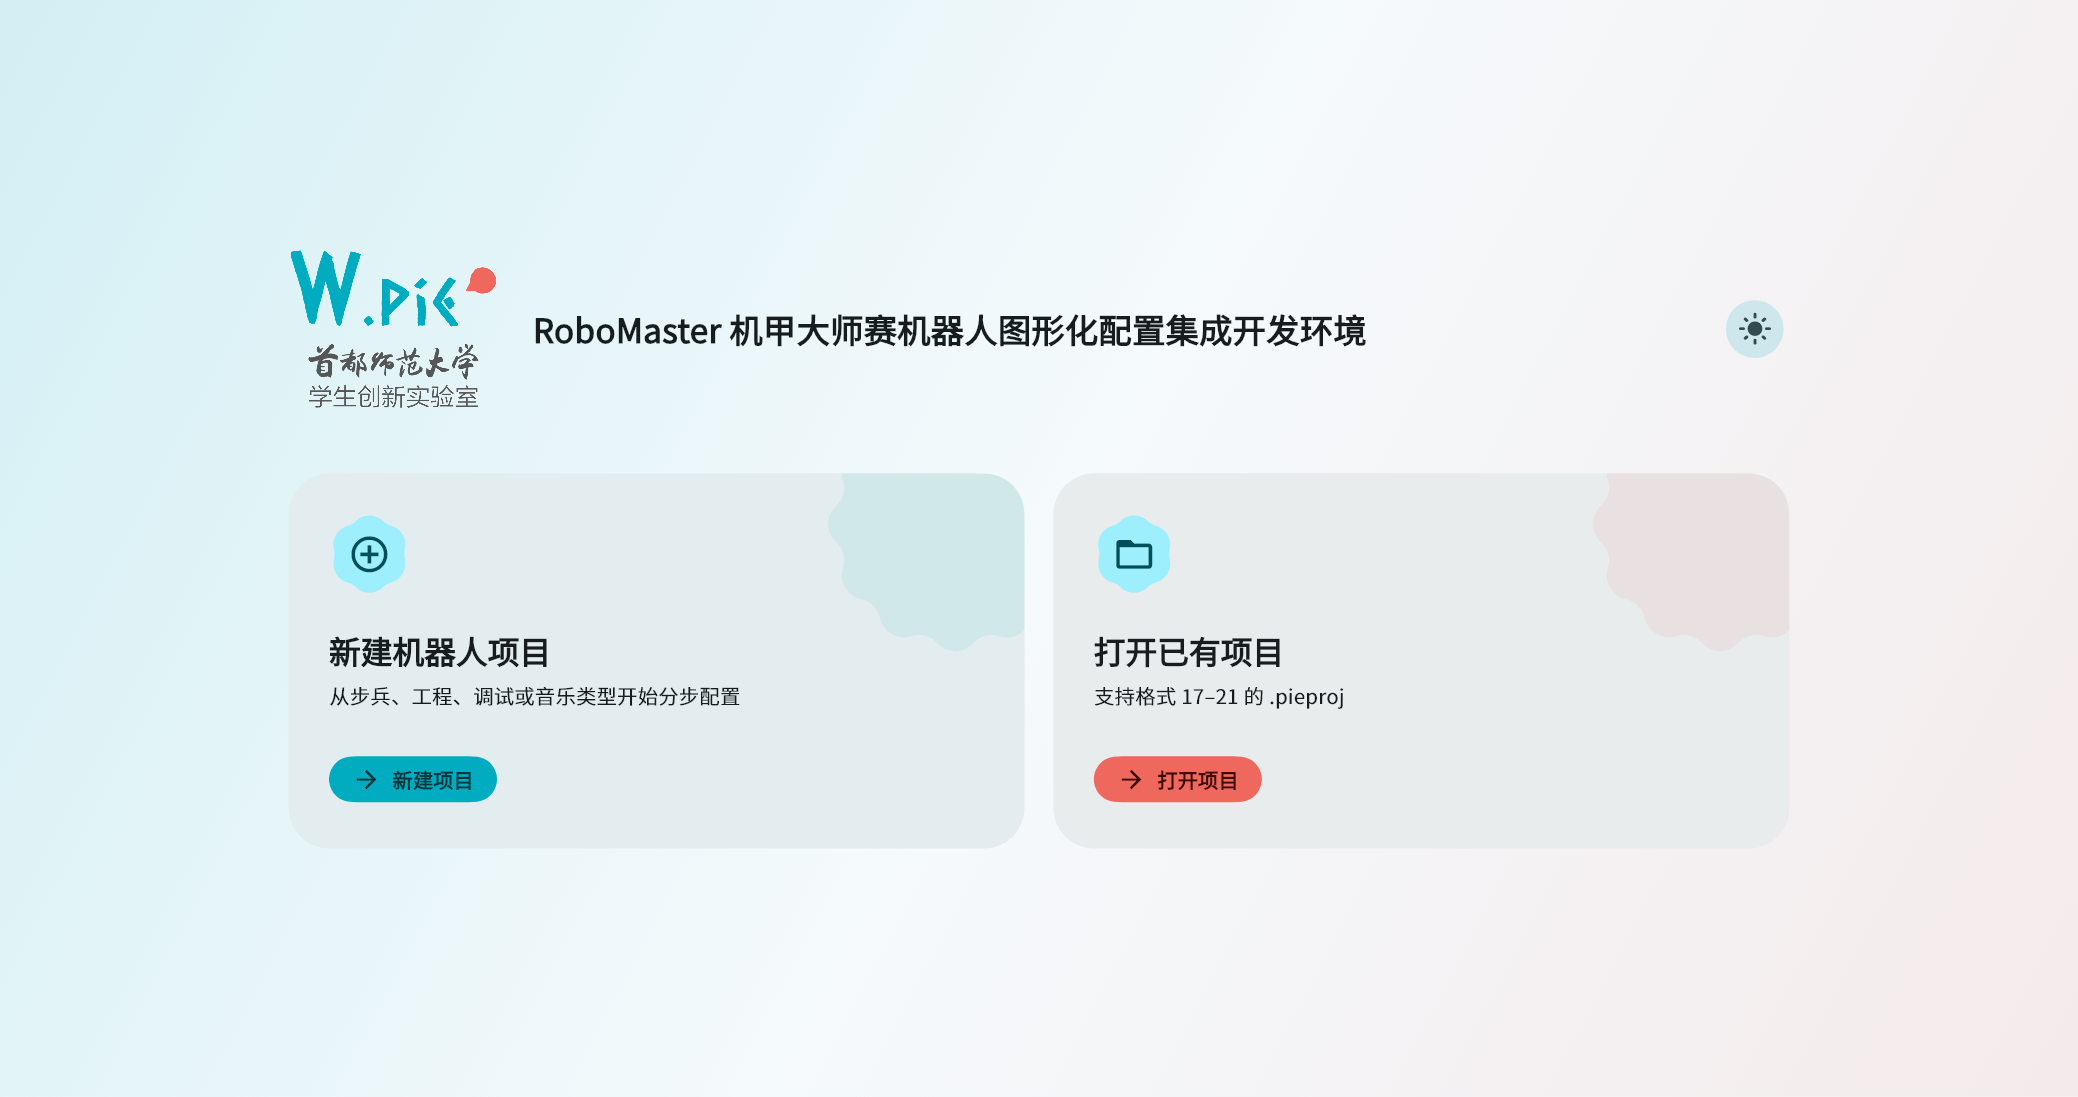
\includegraphics[width=0.92\linewidth]{image/ch01/1-1-home.png}
  \caption{PIE-Block 首页：新建项目、打开已有项目与最近项目}
  \label{fig:concise-home}
\end{figure}

\section{安装与启动}

Windows 提供安装版与免安装版，Linux 提供压缩包，Android 提供安装包；Web 版可以直接在
浏览器中使用。桌面版内置编译工具，安装或解压后即可使用，无需另行安装编译器。首次启动
需要准备运行环境，可能需要短暂等待。

Web 版适合配置项目、执行检查与查看生成结果，不能编译或烧录；编译与烧录应在桌面版完成。

\section{首页与项目文件}

首页提供三个入口（图~\ref{fig:concise-home}）：

\begin{itemize}
  \item \textbf{新建项目}：选择项目类型，填写项目名称与保存位置后创建；
  \item \textbf{打开项目}：选择已有的 \texttt{.pieproj} 文件；
  \item \textbf{最近项目}：按打开顺序列出最近使用的工程，点击即可继续。
\end{itemize}

随书示例工程位于仓库的 \texttt{book/examples/} 目录，可直接导入对照，
见表~\ref{tab:concise-examples}。

\begin{table}[htbp]
  \centering
  \small
  \begin{tabular}{@{}lll@{}}
    \toprule
    示例文件 & 类型 & 用途 \\
    \midrule
    \texttt{infantry-standard.pieproj} & 步兵 & 标准步兵配置 \\
    \texttt{mecanum4.pieproj} & 工程 & 四轮麦克纳姆轮底盘 \\
    \texttt{omni3.pieproj} & 工程 & 三轮全向底盘 \\
    \texttt{arm2dof.pieproj} & 工程 & 二自由度机械臂 \\
    \texttt{debug-checklist.pieproj} & 调试 & 装车前检查单 \\
    \texttt{music-twinkle.pieproj} & 音乐 & 乐曲片段 \\
    \bottomrule
  \end{tabular}
  \caption{随书示例工程}
  \label{tab:concise-examples}
\end{table}

\section{通用流程与安全前提}

四种项目的向导长短不同，但流程一致：填写参数 $\rightarrow$ 检查与摘要 $\rightarrow$
生成代码 $\rightarrow$ 烧录。向导底部的“下一步”逐页推进，已填写的页面显示为完成状态。

“检查与摘要”页把配置中的问题分为两类：

\begin{itemize}
  \item \textbf{错误}：配置不完整或自相矛盾，阻止继续生成。点击条目可跳回对应页面修改；
  \item \textbf{警告}：配置合法但可能不符合预期，只作提醒，不阻止生成。
\end{itemize}

“生成代码”页只读，用于核对配置产生的程序，不需要修改，也不能写回项目文件。实际编译在
“烧录”页完成：连接主控板后点击“编译并烧录”；没有主控板时可用“仅编译”确认配置与编译
环境正常。

\begin{note}
实车操作的安全前提：车体架空、轮子离地；速度临时调低；弹仓清空、射界无人；烧录前关闭
主控板 SERVO、POWER 与机械拓展板 POWER、BOOSTER 四个供电开关；上电后不插拔接线。
只允许烧录主控板，机械拓展板不可烧录。
\end{note}
